\begin{figure}[htbp]
\centering
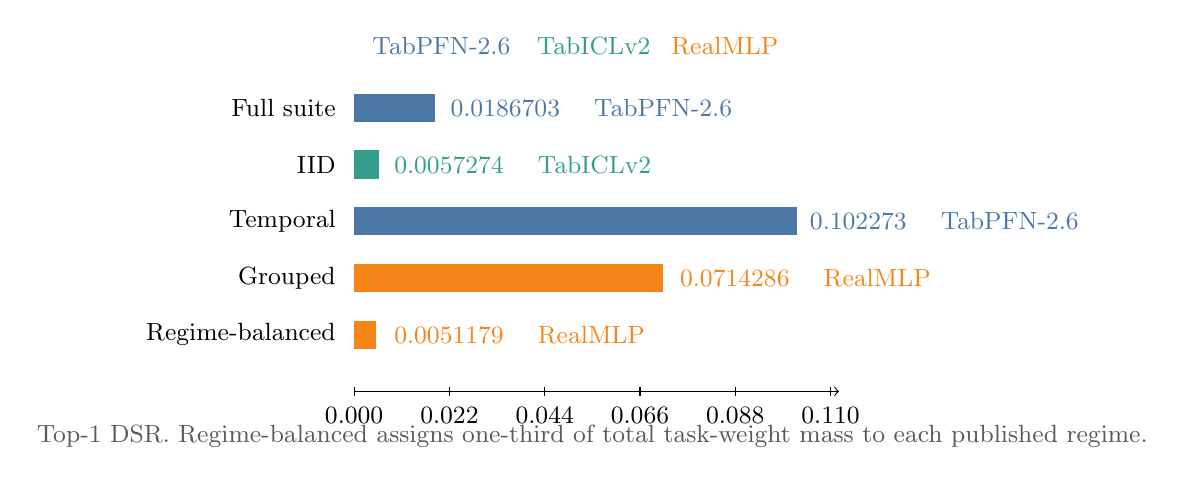
\begin{tikzpicture}[x=55cm,y=0.72cm,font=\small]
  \definecolor{tabpfn}{RGB}{76,120,168}
  \definecolor{tabicl}{RGB}{51,158,140}
  \definecolor{realmlp}{RGB}{245,133,24}
  \draw[->] (0,0) -- (0.112,0);
  \foreach \x/\lab in {0/0.000,0.022/0.022,0.044/0.044,0.066/0.066,0.088/0.088,0.110/0.110}
    {\draw (\x,-0.08)--(\x,0.08) node[below=4pt] {\lab};}
  \node[anchor=east] at (-0.002,5) {Full suite};
  \fill[tabpfn] (0,4.75) rectangle (0.0186703097,5.25);
  \node[anchor=west,text=tabpfn] at (0.020,5) {0.0186703 \quad TabPFN-2.6};
  \node[anchor=east] at (-0.002,4) {IID};
  \fill[tabicl] (0,3.75) rectangle (0.0057274,4.25);
  \node[anchor=west,text=tabicl] at (0.007,4) {0.0057274 \quad TabICLv2};
  \node[anchor=east] at (-0.002,3) {Temporal};
  \fill[tabpfn] (0,2.75) rectangle (0.102273,3.25);
  \node[anchor=west,text=tabpfn] at (0.103,3) {0.102273 \quad TabPFN-2.6};
  \node[anchor=east] at (-0.002,2) {Grouped};
  \fill[realmlp] (0,1.75) rectangle (0.0714286,2.25);
  \node[anchor=west,text=realmlp] at (0.073,2) {0.0714286 \quad RealMLP};
  \node[anchor=east] at (-0.002,1) {Regime-balanced};
  \fill[realmlp] (0,0.75) rectangle (0.0051179,1.25);
  \node[anchor=west,text=realmlp] at (0.007,1) {0.0051179 \quad RealMLP};
  \node[anchor=west,text=tabpfn] at (0,6.1) {$\blacksquare$ TabPFN-2.6};
  \node[anchor=west,text=tabicl] at (0.038,6.1) {$\blacksquare$ TabICLv2};
  \node[anchor=west,text=realmlp] at (0.069,6.1) {$\blacksquare$ RealMLP};
  \node[align=center,text=gray!70!black] at (0.055,-0.8)
  {Top-1 DSR. Regime-balanced assigns one-third of total task-weight mass to each published regime.};
\end{tikzpicture}
\caption{BeyondArena top-1 DSR and nominal winner across the full-suite, IID, temporal, grouped, and regime-balanced analyses. The regime-balanced baseline assigns one-third of total task-weight mass to each published regime.}
\label{fig:beyond-regimes}
\end{figure}

